\documentclass[12pt]{article}
\usepackage[utf8]{inputenc}
\usepackage[spanish]{babel}
\usepackage{amsmath}
\usepackage{amsthm}
\usepackage{multicol,multienum}
\usepackage{graphicx}
\usepackage{float}
\usepackage{tikz}
\usepackage{color}
\usepackage{anysize}
\usepackage{anyfontsize}
\usepackage{geometry}
\usepackage[os=win]{menukeys}
%Este paquete permite manejar los encabezados del documento
\usepackage{fancyhdr}
%hay que definir el ambiente de la página
\pagestyle{fancy}
%aqui va el texto para todas las paginas l--> izquierda, r--> derecha, hay un C--> para centrar el texto deseado
%\lhead{Curso de Física Computacional}
\fancyhead[R]{\nouppercase{\leftmark}}
%define el ancho de la linea que separa el encabezado del cuerpo del texto
\renewcommand{\headrulewidth}{0.5pt}
\setlength{\parskip}{1em}
\renewcommand{\baselinestretch}{1.5}
\interfootnotelinepenalty=8000
\usepackage{hyperref}
%esta parte define el color del marco que aparece en las hiperreferencias.
\definecolor{links}{HTML}{2A1B81}
\hypersetup{colorlinks,linkcolor=,urlcolor=links}
\spanishdecimal{.}
\marginsize{1.5cm}{1.5cm}{1.5cm}{1.5cm}
\author{M. en C. Gustavo Contreras Mayén.}
\title{Instalación de Anaconda 3 \\ \begin{Large} Curso de Física Computacional\end{Large} \\
\begin{small}
\texttt{curso.fisica.comp@gmail.com}
\end{small}}
\date{ }
\begin{document}
\maketitle
\fontsize{14}{14}\selectfont
\section{\texttt{python} para el curso de Física Computacional}
En el curso de Física Computacional manejaremos \texttt{python} como lenguaje de programación, por lo que será necesario contar con un equipo de cómputo para trabajar fuera del laboratorio; a continuación presentamos una guía breve de la instalación de \texttt{Python} en un equipo que opere con Linux, iOS o Windows.
\par
La distribución de Anaconda con \texttt{python} permite la instalación del kernel además de un conjunto de paquetes en un sólo paso al momento de instalar, otra manera de contar con el mismo entorno de Anaconda, sería instalar paquete por paquete, pero hay que tomar en cuenta que un paquete puede requerir de otro (dependencia) y antes de instalar ese paquete, habría que instalar otro(s) inicialmente. La distribución de Anaconda resuelve todo esto y nos evita los conflictos en caso de requerir las dependencias.
\par
Anaconda cuenta con paquetes de instalación para los sistemas operativos Windows, iOS y Linux, en cada caso, hay que revisar la versión del sistema operativo, es decir, si es de 32 o 64 bits, esto es importante dado que optimizamos el uso del procesador en el caso de 64 bits.
\par
La versión de \texttt{python} que se utilizará para el curso, es la 3.6 @ 64 bits, mencionamos que existe una misma versión de \texttt{python} para sistemas operativos a 32 bits. La versión 2.7.x de \texttt{python} aún se encuentra disponible pero prácticamente ya está de salida.
\par
Existen diferencias sintácticas entre ambas versiones, por lo que al anunciar que usaremos la versión 3.6, toda referencia al lenguaje, será para esta versión.
\par
A continuación veremos de manera gráfica el proceso de instalación de Anaconda para cada sistema operativo. Los equipos del Laboratorio de Enseñanza en Cómputo, donde se impartirá la clase, manejan linux @ 64 bits, con Fedora como distribución.
\section{Descargando Anaconda 3}
Para conseguir el archivo de instalación de Anaconda 3\footnote{Versión 4.0.0, liberada el 31 de mayo del 2017, este documento se actualizó en agosto del mismo año.}, será necesario ingresar a la página de \emph{Continuum Analytics}, que es la empresa que se encarga del software, la liga es: \url{https://www.continuum.io/downloads}
\par
Una vez que identificamos el acceso para nuestro sistema operativo, el siguiente paso es descargar el respectivo archivo.
\section{Instalando Anaconda 3}
\subsection{Instalando Anaconda 3 en Windows.}
Podemos utilizar \texttt{python} y las librerías más comunes a partir de una instalación sucesiva de los archivos, requiere que conozcamos la versión del sistema operativo que tengamos en nuestro equipo. Comencemos con una instalación bajo Windows.
\begin{enumerate}
\item Hay que descargar de la página de Anaconda: \url{http://continuum.io/downloads}, la versión de nuestro sistema operativo y la versión 3.6 de p\texttt{python}.
\begin{figure}[H]
	\centering
	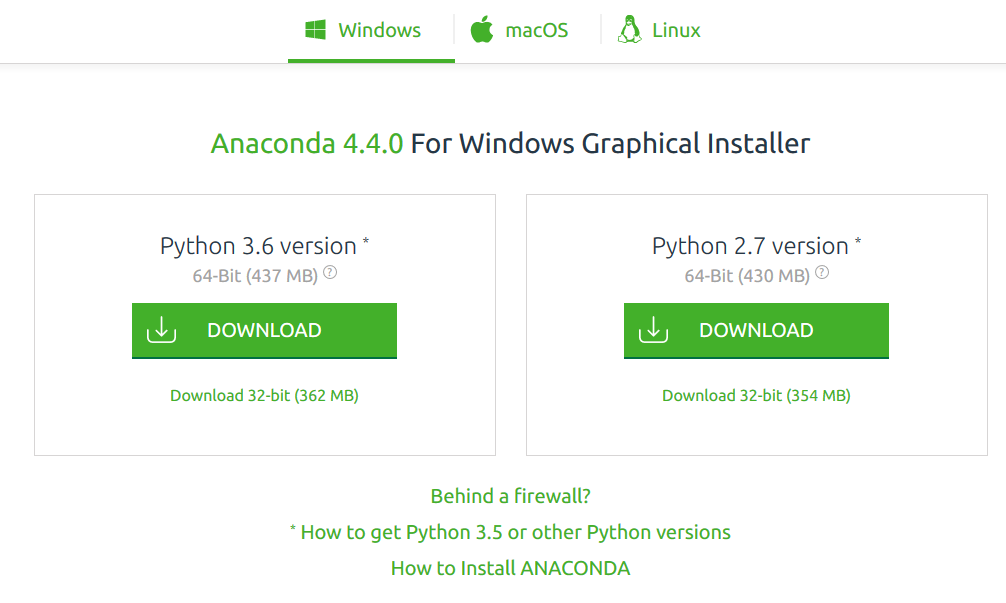
\includegraphics[scale=0.5]{Imagenes/Instalacion_Anaconda_Windows_01} 
\end{figure}
\item Una vez que se completa la descarga, abrimos la carpeta en donde se descargó el archivo ejecutable (*.exe) y hacemos doble click sobre el mismo para iniciar el proceso de instalación.
\begin{figure}[H]
	\centering
	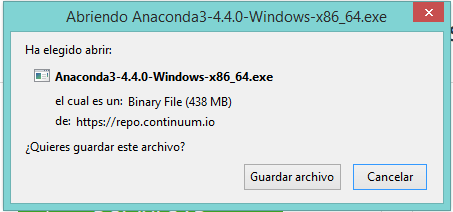
\includegraphics[scale=0.5]{Imagenes/Instalacion_Anaconda_Windows_02}
\end{figure}
\item Se presenta la ventana de Bienvenida en donde se nos avisa que se dará inicio al proceso de instalación de Anaconda 3 en  Windows.
\begin{figure}[H]
	\centering
	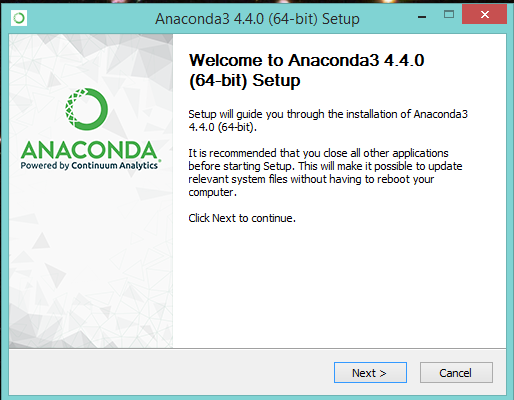
\includegraphics[scale=0.5]{Imagenes/Instalacion_Anaconda_Windows_03} 
\end{figure}
\item Se acepta la licencia de uso de la distribución.
\begin{figure}[H]
	\centering
	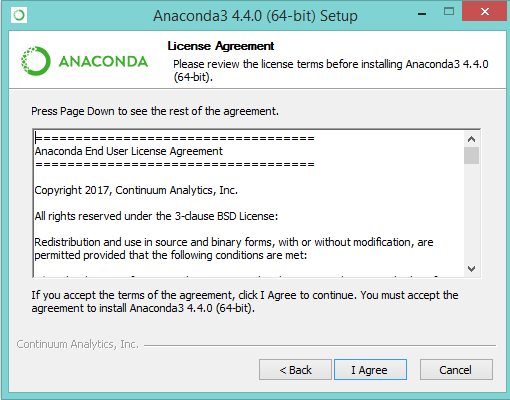
\includegraphics[scale=0.5]{Imagenes/Instalacion_Anaconda_Windows_04} 
\end{figure}
\item En el caso de que tu equipo bajo Windows tenga varios usuarios, hay que definir si se permite la ejecución para todos los usuarios o sólo para el que está realizando la instalación, Anaconda 3 recomienda que sea sólo al usuario que instala, de lo contrario hay que dar permisos de administrador (a menos que seas un usuario avanzado de Windows, sabrás lo que implica esta tarea)
\begin{figure}[H]
	\centering
	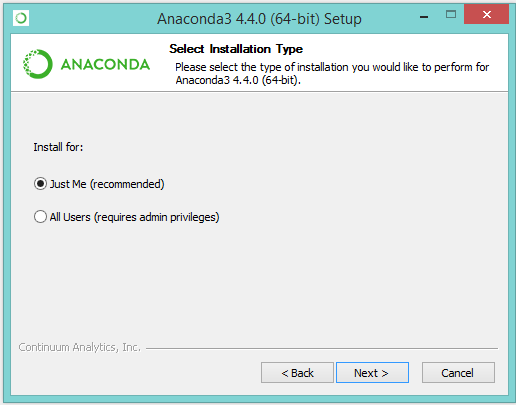
\includegraphics[scale=0.5]{Imagenes/Instalacion_Anaconda_Windows_05} 
\end{figure}
\item Se nos pregunta por las carpetas de instalación, indicando las que se manejan por defecto, se recomienda no modificar la ruta.
\begin{figure}[H]
	\centering
	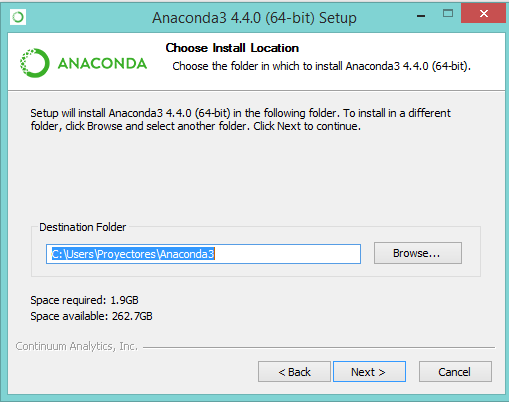
\includegraphics[scale=0.5]{Imagenes/Instalacion_Anaconda_Windows_06} 
\end{figure}
\item Opciones de instalación avanzadas, se deja tal cual se presenta en la ventana, es decir, sólo queda activada la opción de \emph{Registrar Anaconda como programa para \texttt{python 3.6}}. Esto asocia la apertura de archivos \texttt{*.py} (archivos de código de \texttt{python} con la distribución Anaconda 3.
\begin{figure}[H]
	\centering
	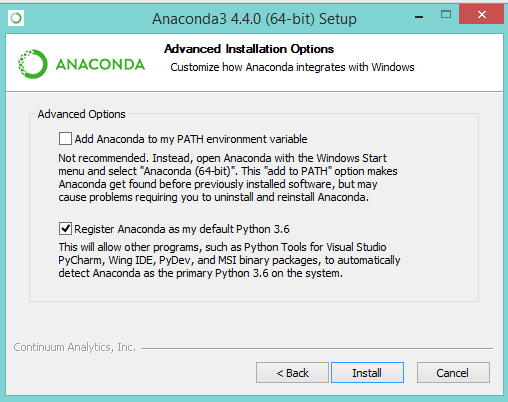
\includegraphics[scale=0.5]{Imagenes/Instalacion_Anaconda_Windows_07} 
\end{figure}
\item Veremos el proceso de instalación a través de una barra de avance de la instalación, dependiendo del equipo, el tiempo de instalación es variable, pero sin contratiempos.
\begin{figure}[H]
	\centering
	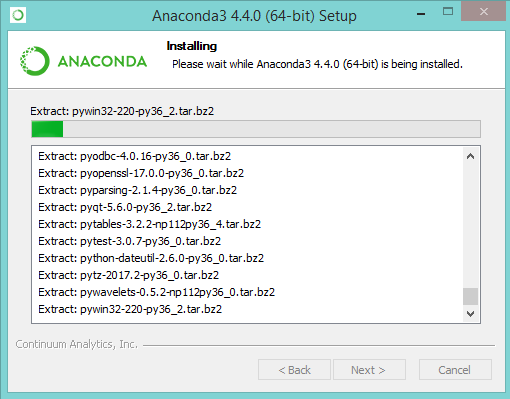
\includegraphics[scale=0.5]{Imagenes/Instalacion_Anaconda_Windows_08} 
\end{figure}
\item Al concluir la instalación, se nos avisa que ha concluido el proceso.
\begin{figure}[H]
	\centering
	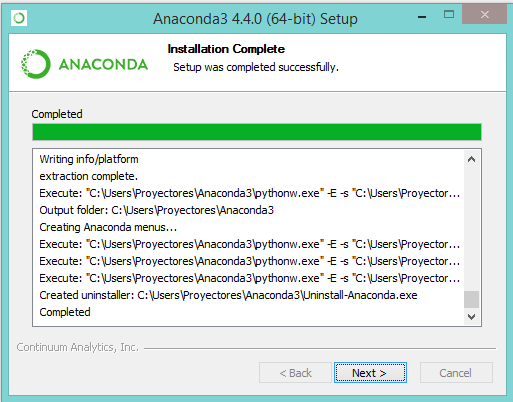
\includegraphics[scale=0.5]{Imagenes/Instalacion_Anaconda_Windows_09} 
\end{figure}
\item La última ventana es una de agradecimiento por utilizar el softwate de Continuum Analytics.
\begin{figure}[H]
	\centering
	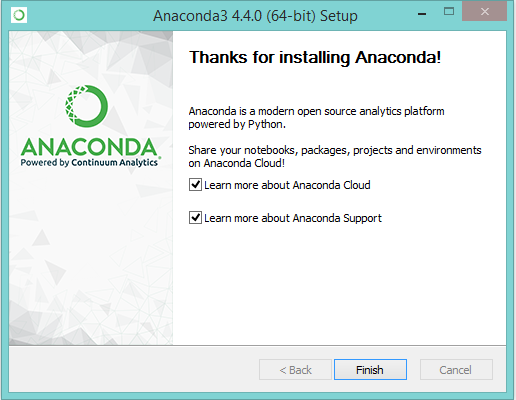
\includegraphics[scale=0.5]{Imagenes/Instalacion_Anaconda_Windows_10} 
\end{figure}
\item Con la instalación completa ya tenemos disponible y listo para usar en nuestro equipo Anaconda.
\begin{figure}[H]
	\centering
	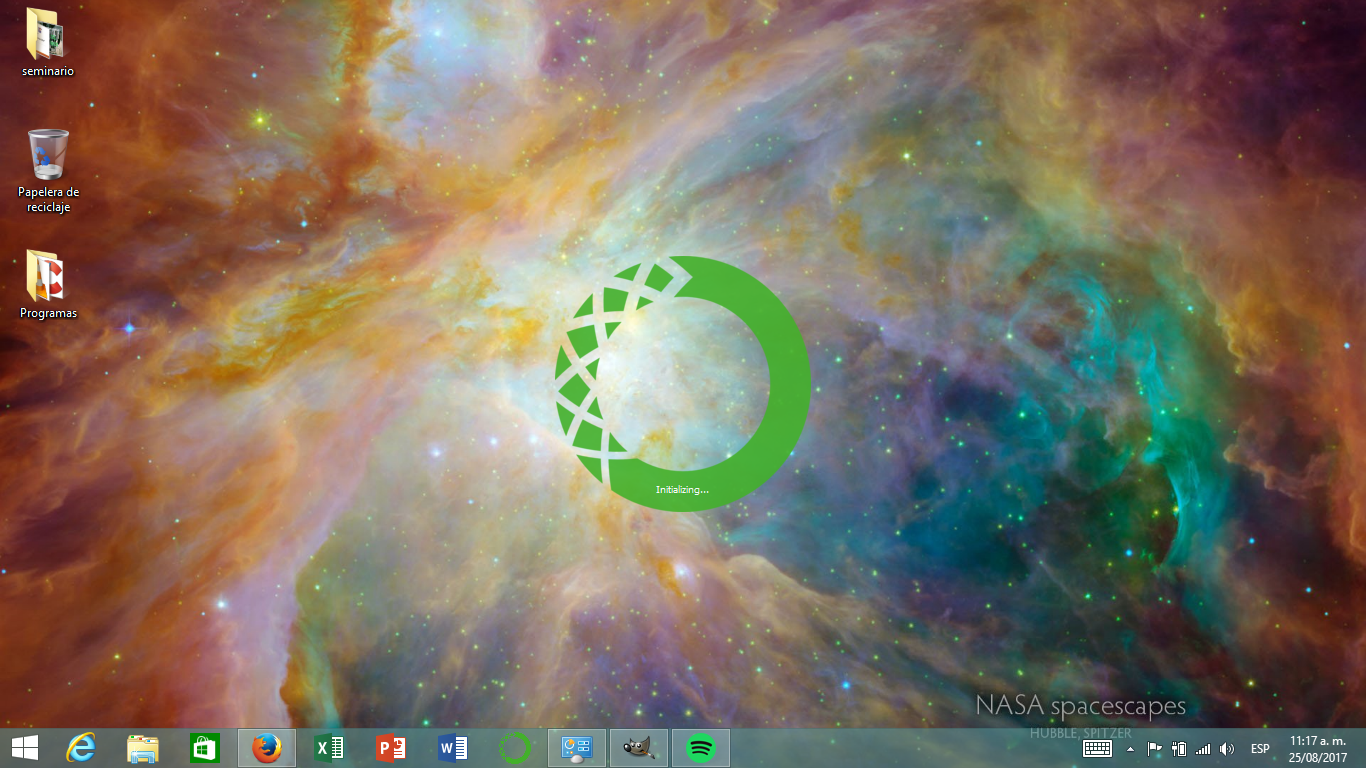
\includegraphics[scale=0.25]{Imagenes/Instalacion_Anaconda_Windows_11} 
\end{figure}
\item Una vez que se ha cargado Anaconda 3, tendremos disponibles los programas de la suite. No olvides actualizar al momento cada de uno de ellos. Nos daremos cuenta cuando se pide una actualización, ya que aparece una flecha junto al engrane de cada programa (esquina superior derecha), ahí elegimos la opción de actualización.
\begin{figure}[H]
	\centering
	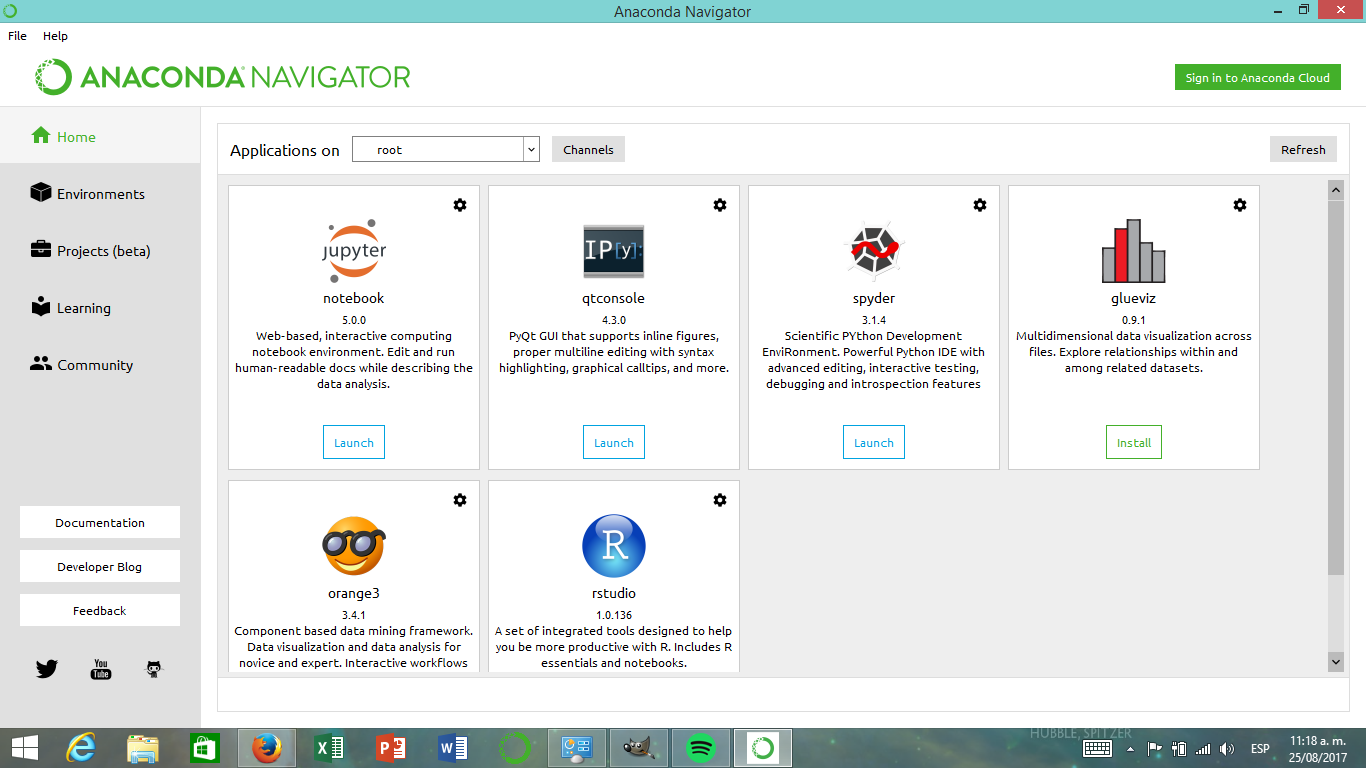
\includegraphics[scale=0.25]{Imagenes/Instalacion_Anaconda_Windows_12} 
\end{figure}
\end{enumerate}
\subsection{Instalando Anaconda en iOS (Mac).}
El sistema operativo iOS cuenta con una interfaz gŕafica bastante cómoda para la instalación de programas y aplicaciones.
\par
Aunque también se puede hacer la instalación de Anaconda 3 mediante la terminal de comandos\footnote{El procedimiento es muy parecido a la instalación en linux, pero lo dejamos a criterio del usuario de un equipo con iOS}, presentaremos el proceso con un instalador gráfico.
\begin{enumerate}
\item Hay que descargar de la página de Anaconda: \url{http://continuum.io/downloads}, la versión de nuestro sistema operativo\footnote{En este ejemplo, la instalación se revisa en un equipo con MacOs X 10.11 El Capitán}, y elegimos el archivo con la versión 3.6.
\begin{figure}[H]
	\centering
	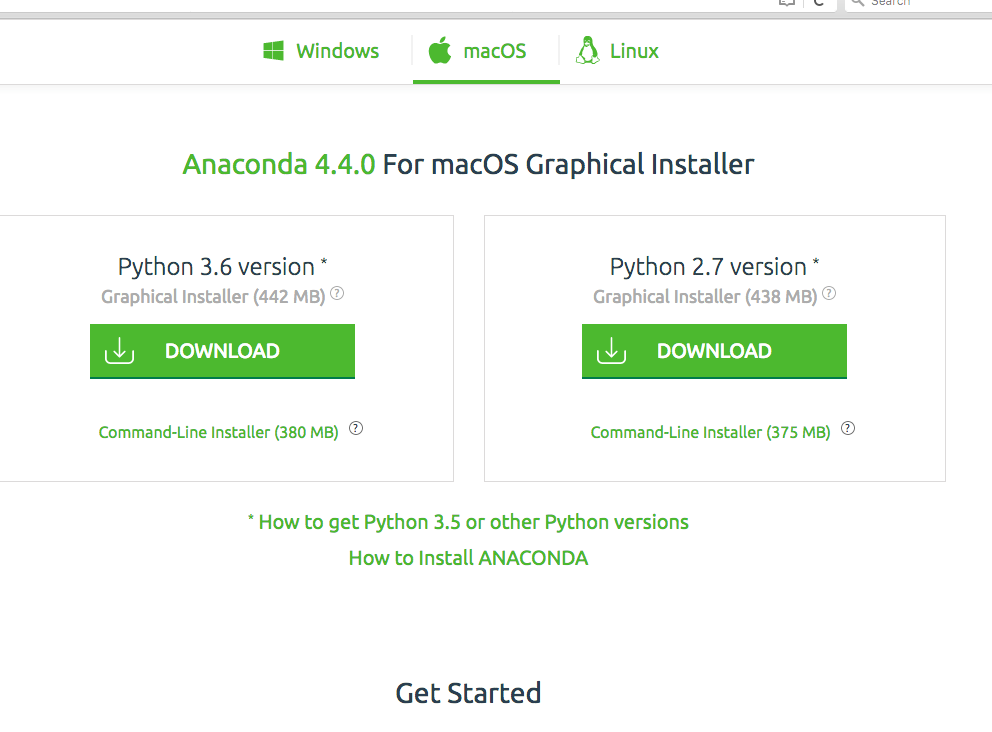
\includegraphics[scale=0.25]{Imagenes/Instalacion_Anaconda_01_iOS_02} 
\end{figure}
\item El archivo que se descarga es del tipo .pkg, que el propio sistema operativo reconoce como un archivo de instalación, basta con hacer doble click sobre el mismo, para iniciar el proceso.
\begin{figure}[H]
	\centering
	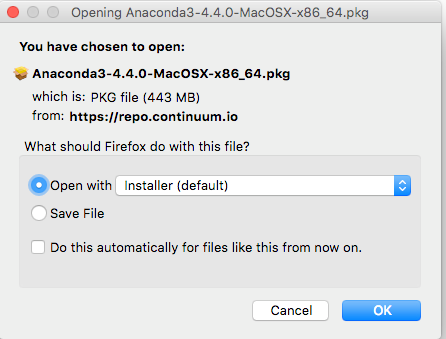
\includegraphics[scale=0.5]{Imagenes/Instalacion_Anaconda_01_iOS_03} 
\end{figure}
\item Se inicia la instalación, en la ventana que se muestra, nos indicará el paso en el que se encuentra el proceso.
\begin{figure}[H]
	\centering
	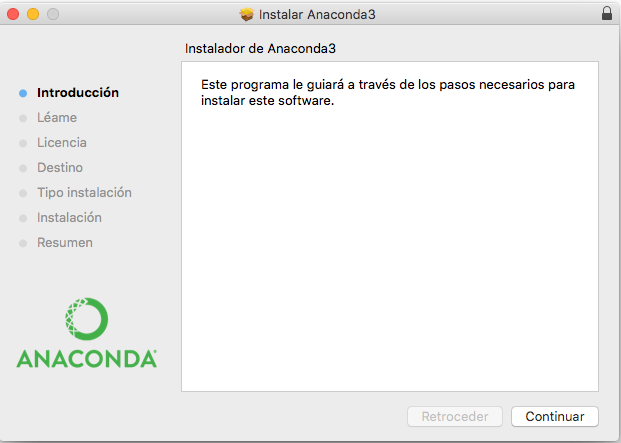
\includegraphics[scale=0.5]{Imagenes/Instalacion_Anaconda_01_iOS_04} 
\end{figure}
\item Se recomienda siempre leer la información que proporciona el proveedor del software, es una tarea que debe de atenderse y ahorrarse problemas posteriores, sobre todo en la parte de lo que el proveedor dice que su software realiza.
\begin{figure}[H]
	\centering
	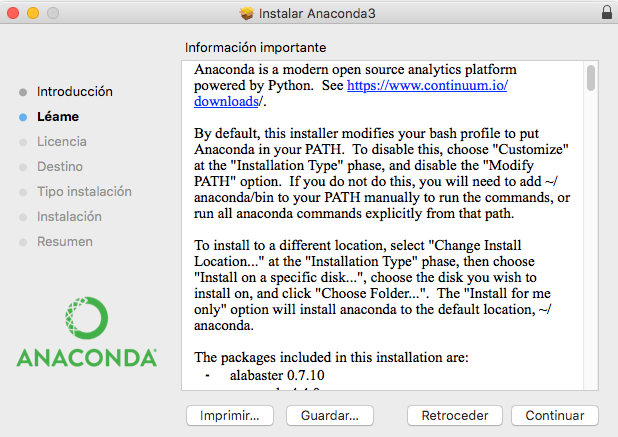
\includegraphics[scale=0.5]{Imagenes/Instalacion_Anaconda_01_iOS_05} 
\end{figure}
\item Se da continuar hasta llegar a la opción de aceptar la Licencia de uso de la distribución, se da continuar y aparecerá una pantalla que demanda aceptar la licencia, se puede imprimir el documento ya sea de manera física o a un archivo.
\begin{figure}[H]
	\centering
	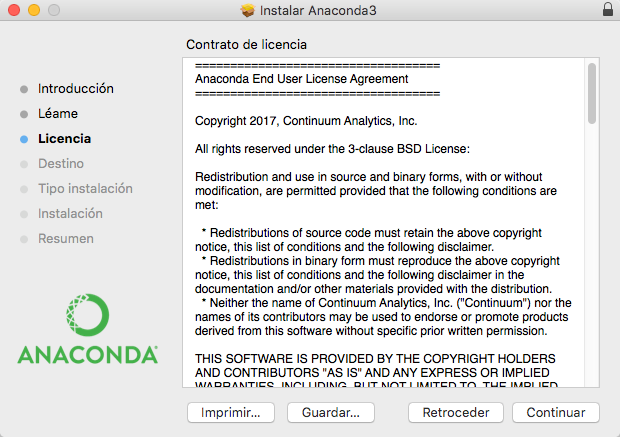
\includegraphics[scale=0.5]{Imagenes/Instalacion_Anaconda_01_iOS_06} 
\end{figure}
\item Se selecciona por defecto la carpeta donde se instalarán los archivos de Anaconda 3, a menos que seas un usuario experto, puedes modificar las rutas.
\begin{figure}[H]
	\centering
	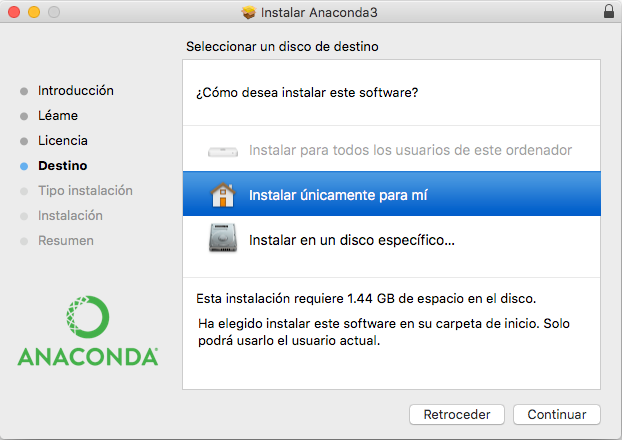
\includegraphics[scale=0.5]{Imagenes/Instalacion_Anaconda_01_iOS_07} 
\end{figure}
\item El tipo de instalación se refiere al(los) usuario(s) que podrán utilizar el programa, a menos que tu equipo de cómputo sea compartido, siempre se recomienda que no haya cambios en las opciones por defecto que se nos muestran.
\begin{figure}[H]
	\centering
	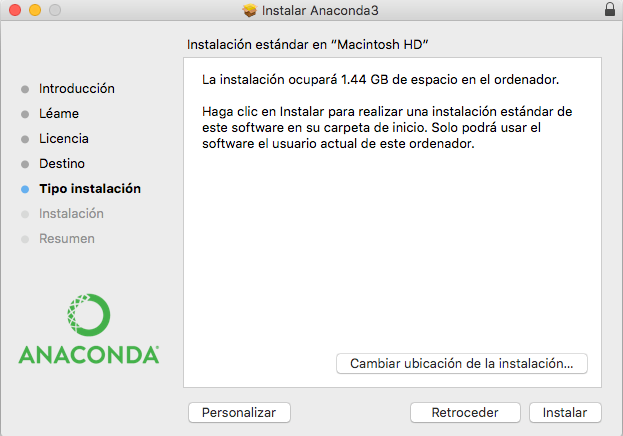
\includegraphics[scale=0.5]{Imagenes/Instalacion_Anaconda_01_iOS_08} 
\end{figure}
\item Se inicia el proceso de la instalación:
\begin{figure}[H]
	\centering
	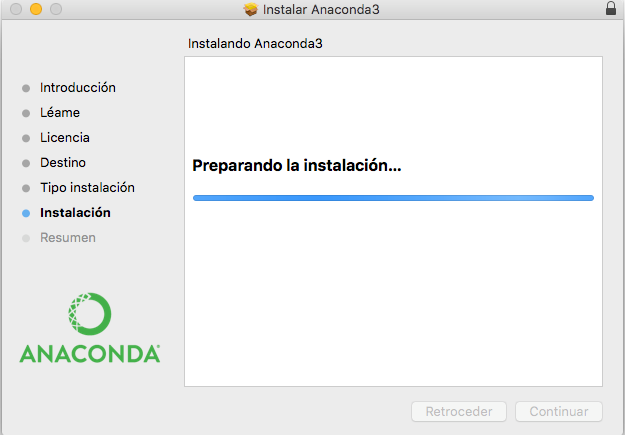
\includegraphics[scale=0.5]{Imagenes/Instalacion_Anaconda_01_iOS_09} 
\end{figure}
\item Mediante una barra de avance en la instalación, veremos que el proceso puede tardar un poco en la instalación. Recomendamos no realizar alguna otra tarea en el equipo para favorecer el proceso y reducir el tiempo de la instalación.
\begin{figure}[H]
	\centering
	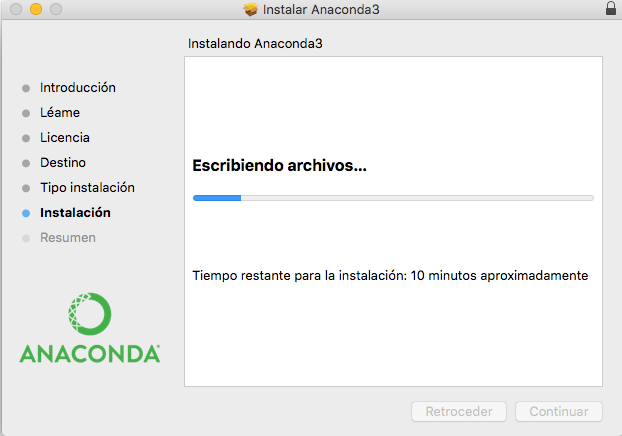
\includegraphics[scale=0.5]{Imagenes/Instalacion_Anaconda_01_iOS_10} 
\end{figure}
 \item Una vez que se completó la instalación, se muestra en pantalla con el aviso.
\begin{figure}[H]
	\centering
	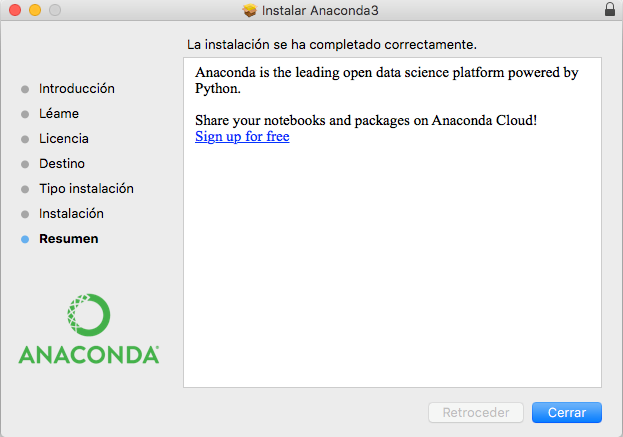
\includegraphics[scale=0.5]{Imagenes/Instalacion_Anaconda_01_iOS_11} 
\end{figure}
\item Tenemos ahora en el dash, el ícono de acceso a Anaconda 3, por lo que ya podremos hacer doble click para que se inicie el programa
\begin{figure}[H]
	\centering
	
\includegraphics[scale=0.15]{Imagenes/Instalacion_Anaconda_01_iOS_12} 
\end{figure}
\item Se nos presenta la interfaz de Anaconda 3 con los programas que ya están instalados y por tanto, podemos utilizarlos.
\begin{figure}[H]
	\centering
	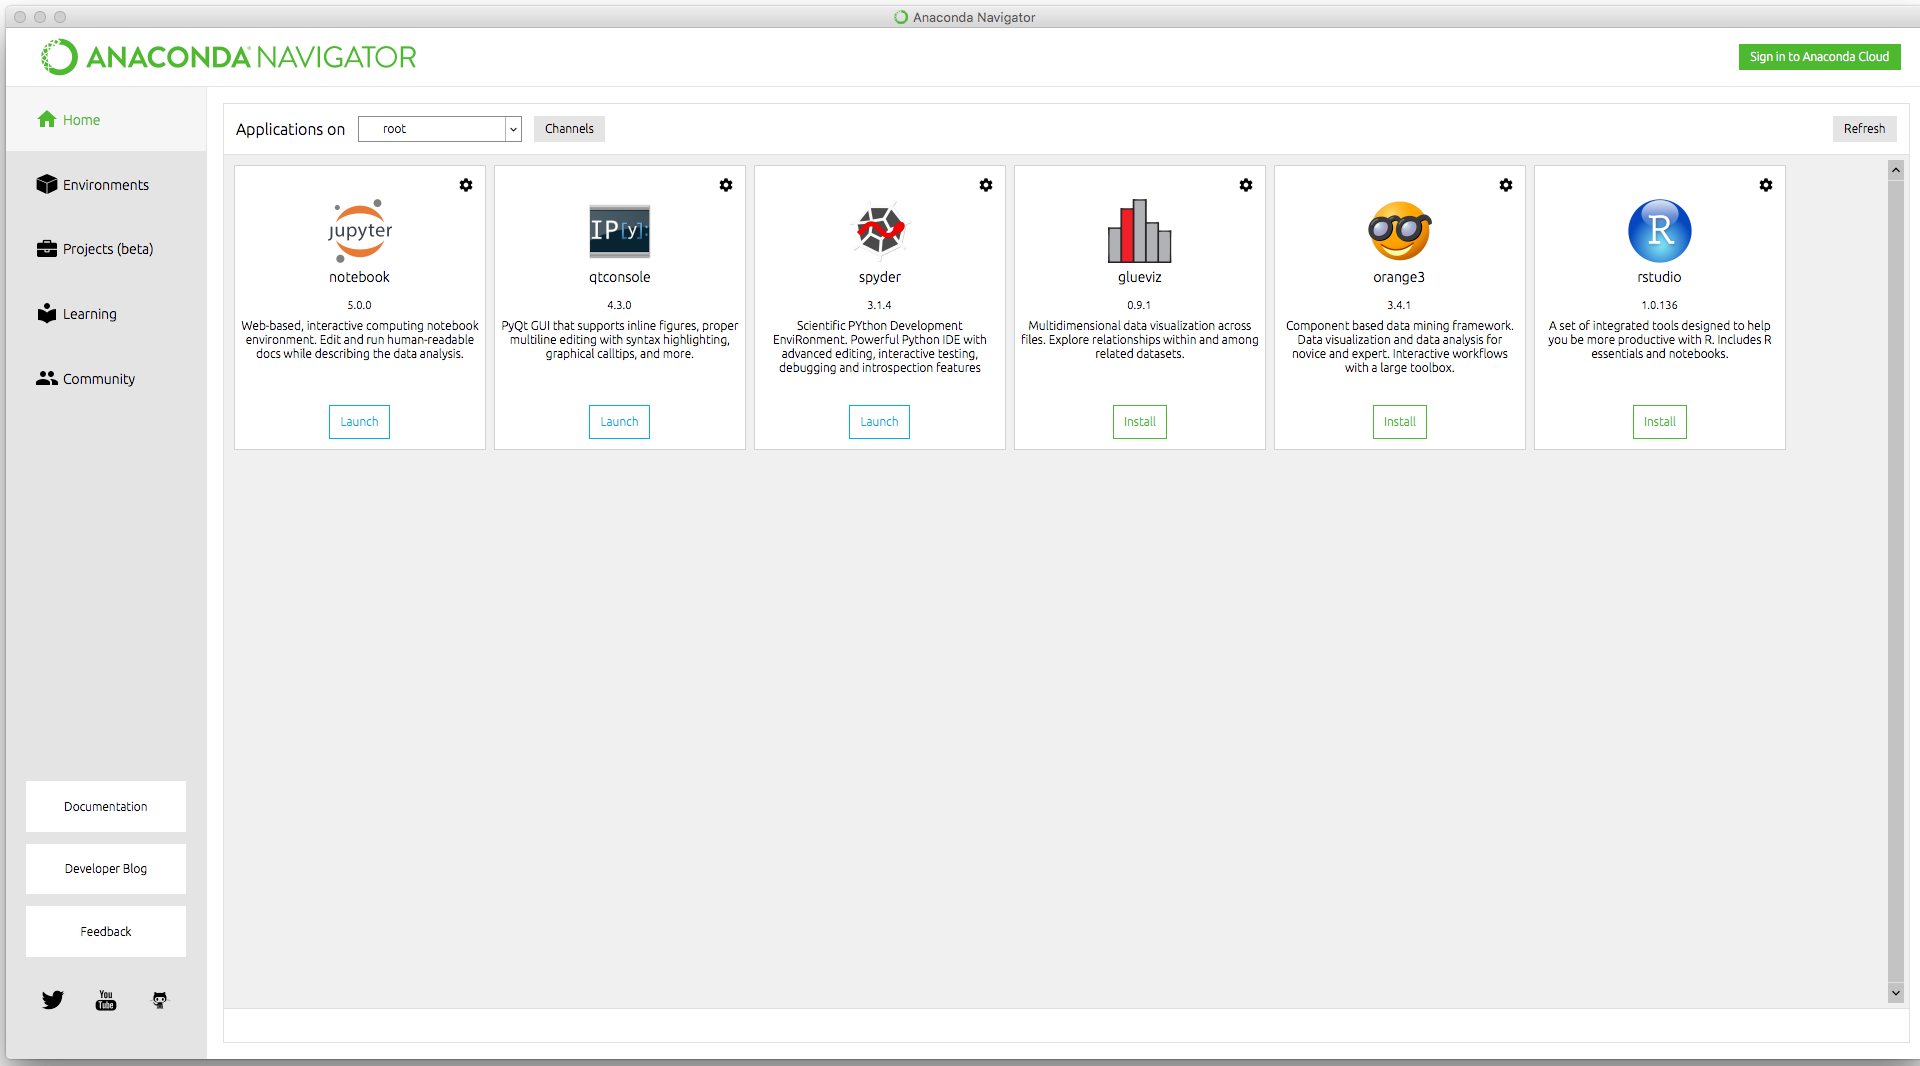
\includegraphics[scale=0.15]{Imagenes/Instalacion_Anaconda_01_iOS_13} 
\end{figure}
\end{enumerate}
\subsection{Instalando Anaconda en Linux}
 La instalación de Anaconda 3 en linux\footnote{En un equipo con Fedora como distribución} se realiza mediante una terminal, los pasos no son complicados, pero hay que tener cuidado con lo que se escribe, tanto para evitar un error o realizar una tarea que ya no se pueda corregir.
\begin{enumerate}
\item El primer paso es descargar la versión 3.6 que corresponda con nuestra distribución de linux, ya sea de 32 bits o 64 bits
\begin{figure}[H]
	\centering
 	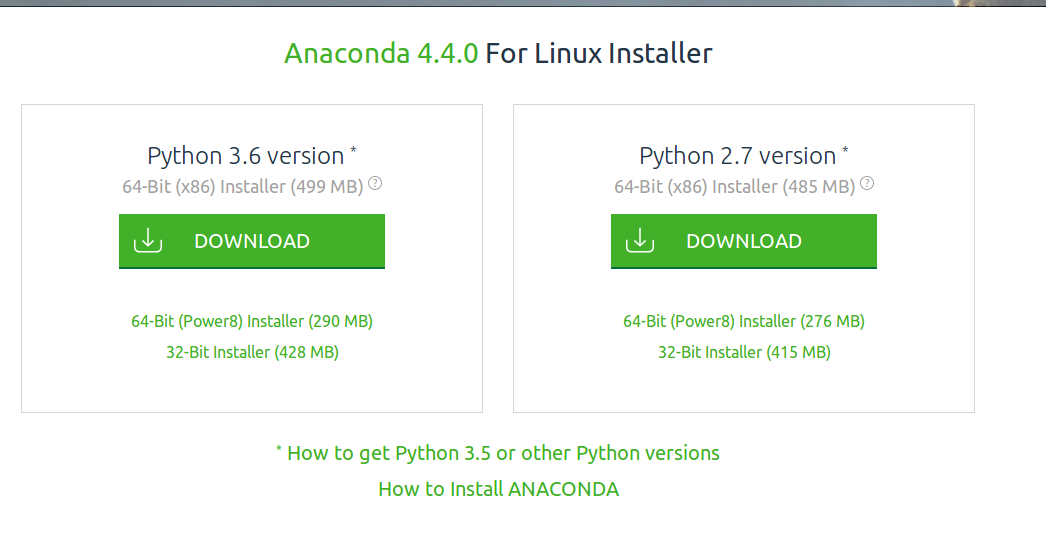
\includegraphics[scale=0.35]{Imagenes/Instalacion_Anaconda_01_linux_01} 
\end{figure}
\item El siguiente paso es descargar el archivo en el equipo
\begin{figure}[H]
 	\centering
 	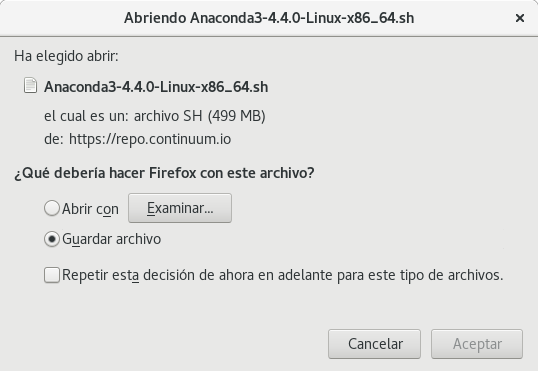
\includegraphics[scale=0.35]{Imagenes/Instalacion_Anaconda_01_linux_02}
\end{figure}
\item Cuando haya concluido la descarga del archivo, habrá que realizar la instalación mediante una terminal de comandos, de acuerdo a la documentación, se necesita una instrucción en la terminal para ello
\begin{figure}[H]
 	\centering
 	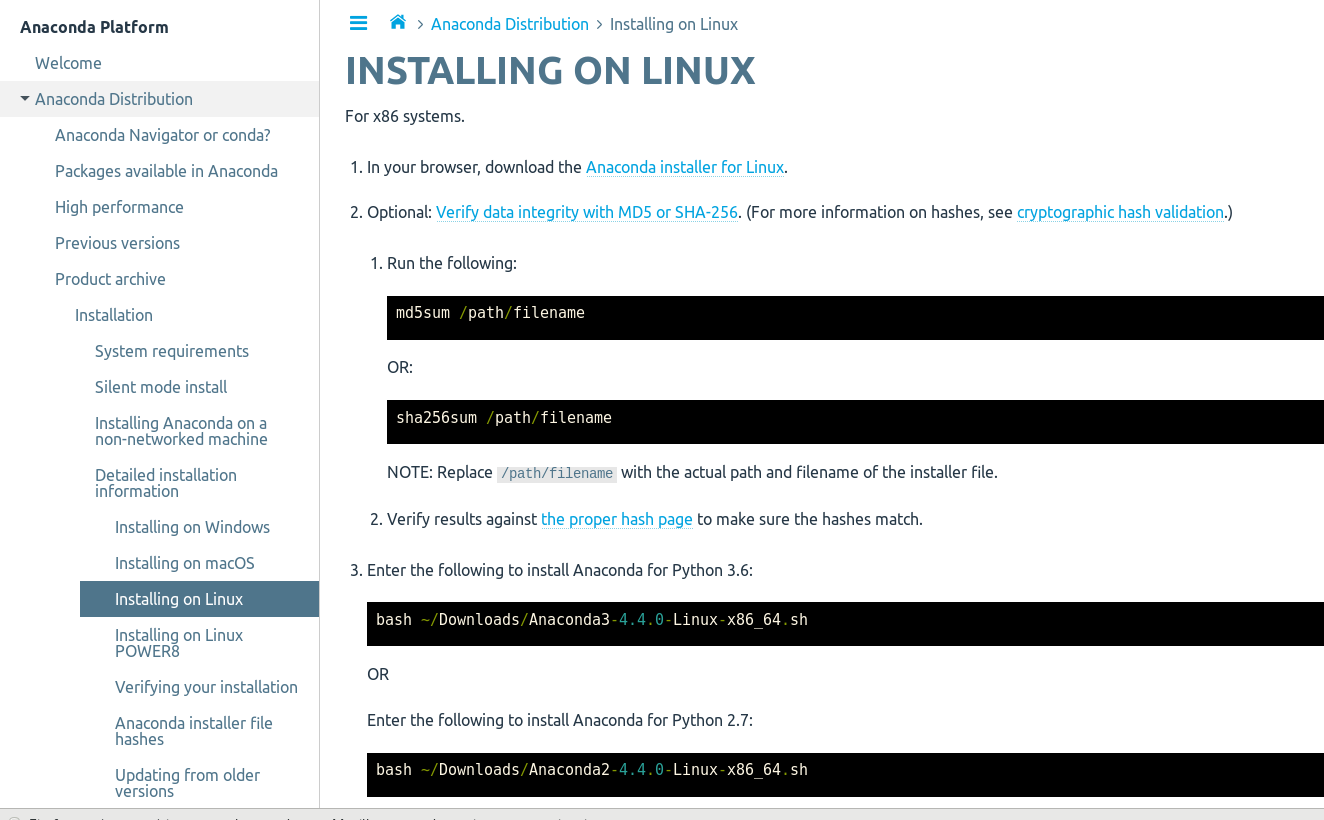
\includegraphics[scale=0.35]{Imagenes/Instalacion_Anaconda_01_linux_03}
\end{figure}
Abrimos una terminal de linux al hacer una combinación de teclas \keys{\ctrl + \Alt + t}, donde escribimos el comando
\\
\begin{verbatim}
bash ~/Descargas/Anaconda3-4.0.0-Linux-x86_64.sh
\end{verbatim}
Toma en cuenta que el nombre del archivo que has descargado, puede ser diferente, por ello verifica antes de teclear el comando.
\begin{figure}[H]
 	\centering
 	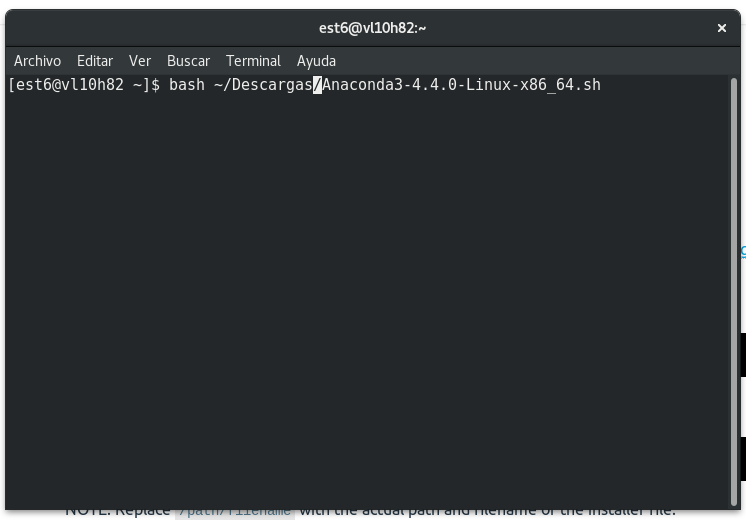
\includegraphics[scale=0.35]{Imagenes/Instalacion_Anaconda_01_linux_04}
\end{figure}
\item Para iniciar la instalación en nuestro equipo, basta con que tecleemos \texttt{Enter}, y se inicie el proceso.
\begin{figure}[H]
 	\centering
 	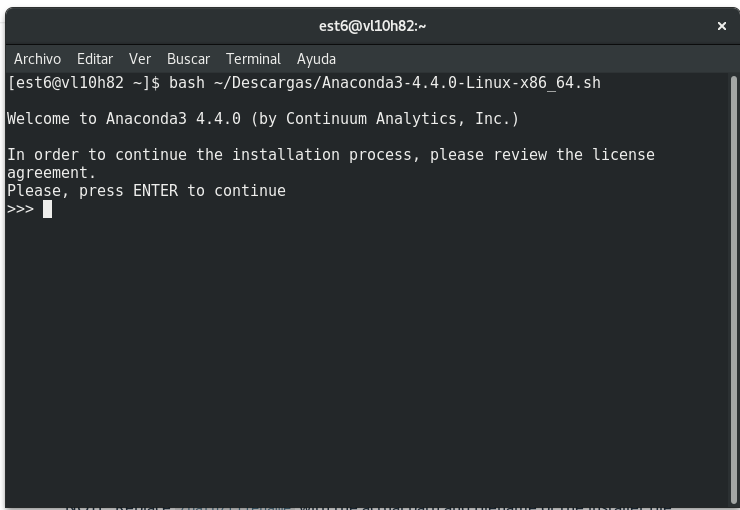
\includegraphics[scale=0.35]{Imagenes/Instalacion_Anaconda_01_linux_05}
\end{figure}
\item Se nos presenta la Licencia de Uso, como en los sistemas operativos anteriores, debemos de revisar la documentación.
\begin{figure}[H]
 	\centering
 	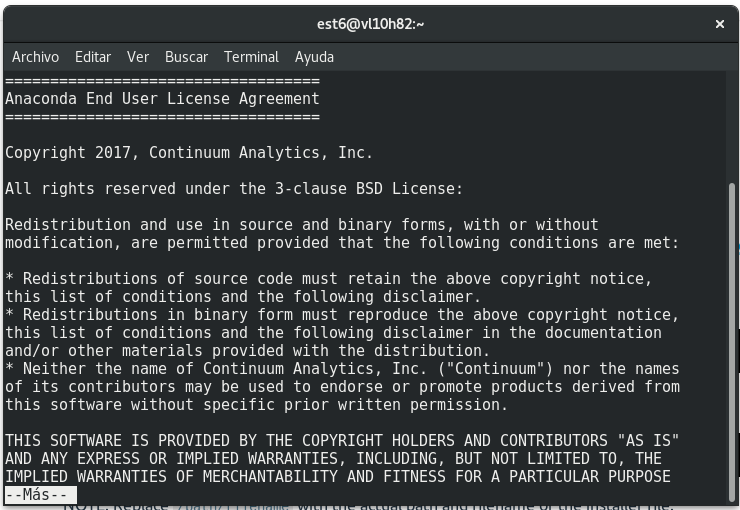
\includegraphics[scale=0.35]{Imagenes/Instalacion_Anaconda_01_linux_06}
\end{figure}
\item La siguiente etapa es definir la ruta en donde se va a instalar el programa, recomendamos altamente que no se modifiquen la ruta de instalación, por lo que tecleamos \keys{\return} (la tecla \texttt{Enter}) para aceptar la ruta por defecto.
\begin{figure}[H]
 	\centering
 	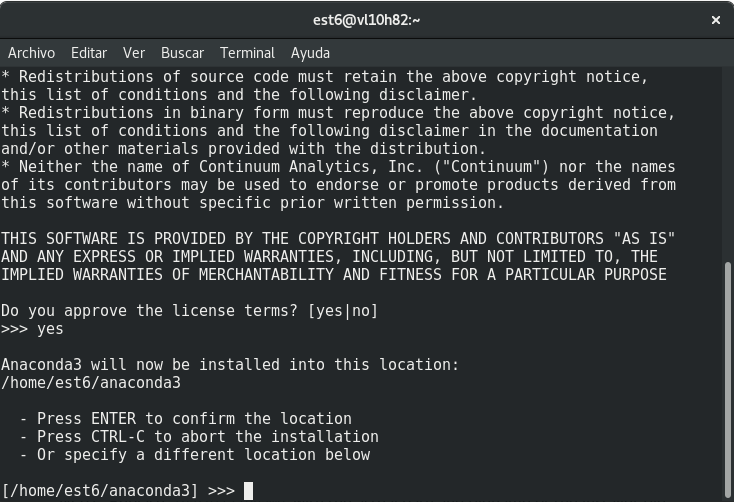
\includegraphics[scale=0.35]{Imagenes/Instalacion_Anaconda_01_linux_07}
\end{figure}
\item Veremos en la terminal, la instalación de los paquetes de manera automática. Una ventaja de usar una plataforma como Anaconda es que los programas, paquetes y librerías ya llevan las referencias necesarias, en caso de que se haga una instalación por separado de cada elemento, lo más seguro es que se requieran y se resuelvan las dependencias necesarias, proceso que puede ser muy tedioso.
\begin{figure}[H]
 	\centering
 	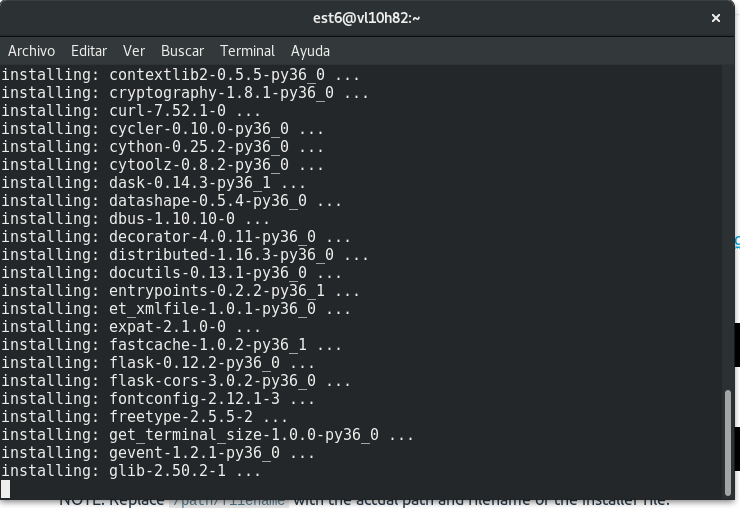
\includegraphics[scale=0.35]{Imagenes/Instalacion_Anaconda_01_linux_08}
\end{figure}
\item Para configurar la ejecución de \texttt{python} desde cualquier punto, hay que ajustar el \texttt{PATH} en el respectivo archivo de linux, por lo que aceptamos el ajuste al archivo.
\begin{figure}[H]
 	\centering
 	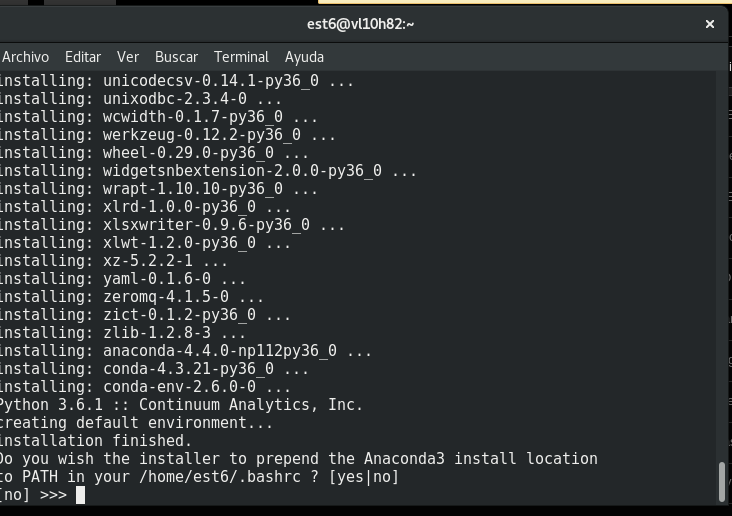
\includegraphics[scale=0.35]{Imagenes/Instalacion_Anaconda_01_linux_09}
\end{figure}
\item Al concluir el proceso de instalación, nos damos cuenta cuando recuperamos el \texttt{promtp} de la terminal de linux.
\begin{figure}[H]
 	\centering
 	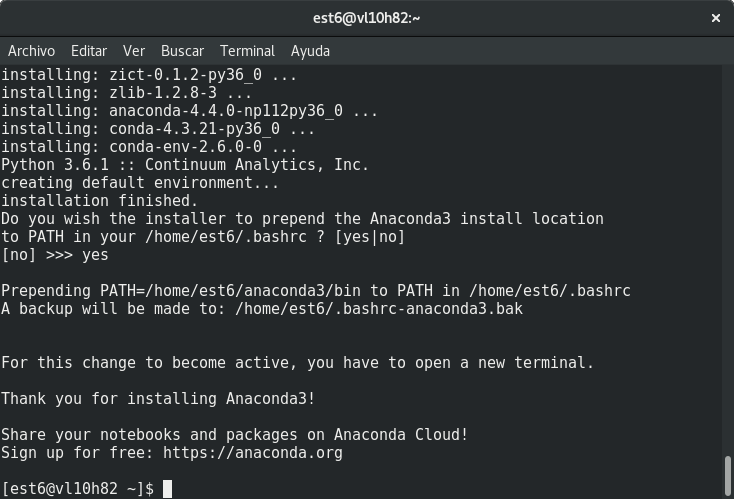
\includegraphics[scale=0.35]{Imagenes/Instalacion_Anaconda_01_linux_10}
\end{figure}
\item Para iniciar el programa, se requiere cerrar la ventana de la terminal en la que hemos trabajado, ya que se reinicia la terminal y se ejecutará sin problemas el programa.
\begin{figure}[H]
 	\centering
 	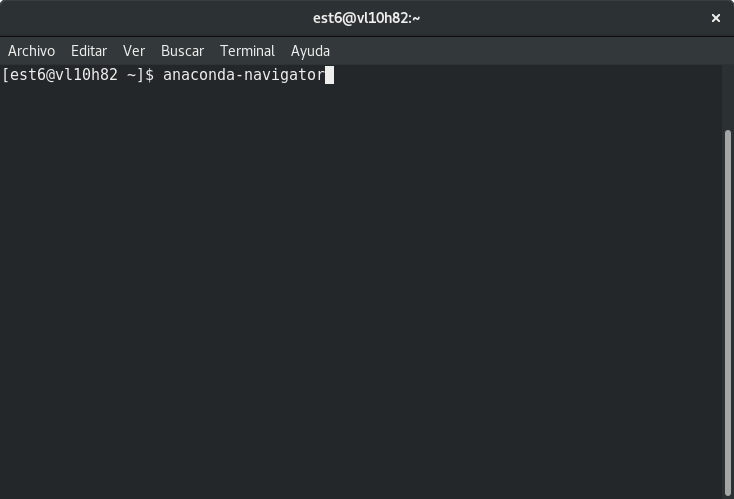
\includegraphics[scale=0.35]{Imagenes/Instalacion_Anaconda_01_linux_11}
\end{figure}
Podrás hacer un enlace simbólico para que tengas el ícono de acceso ya sea en el escritorio o en la barra de tareas.
\item Vemos ahora el entorno de Anaconda 3 correctamente instalado en nuestro equipo con linux.
\begin{figure}[H]
 	\centering
 	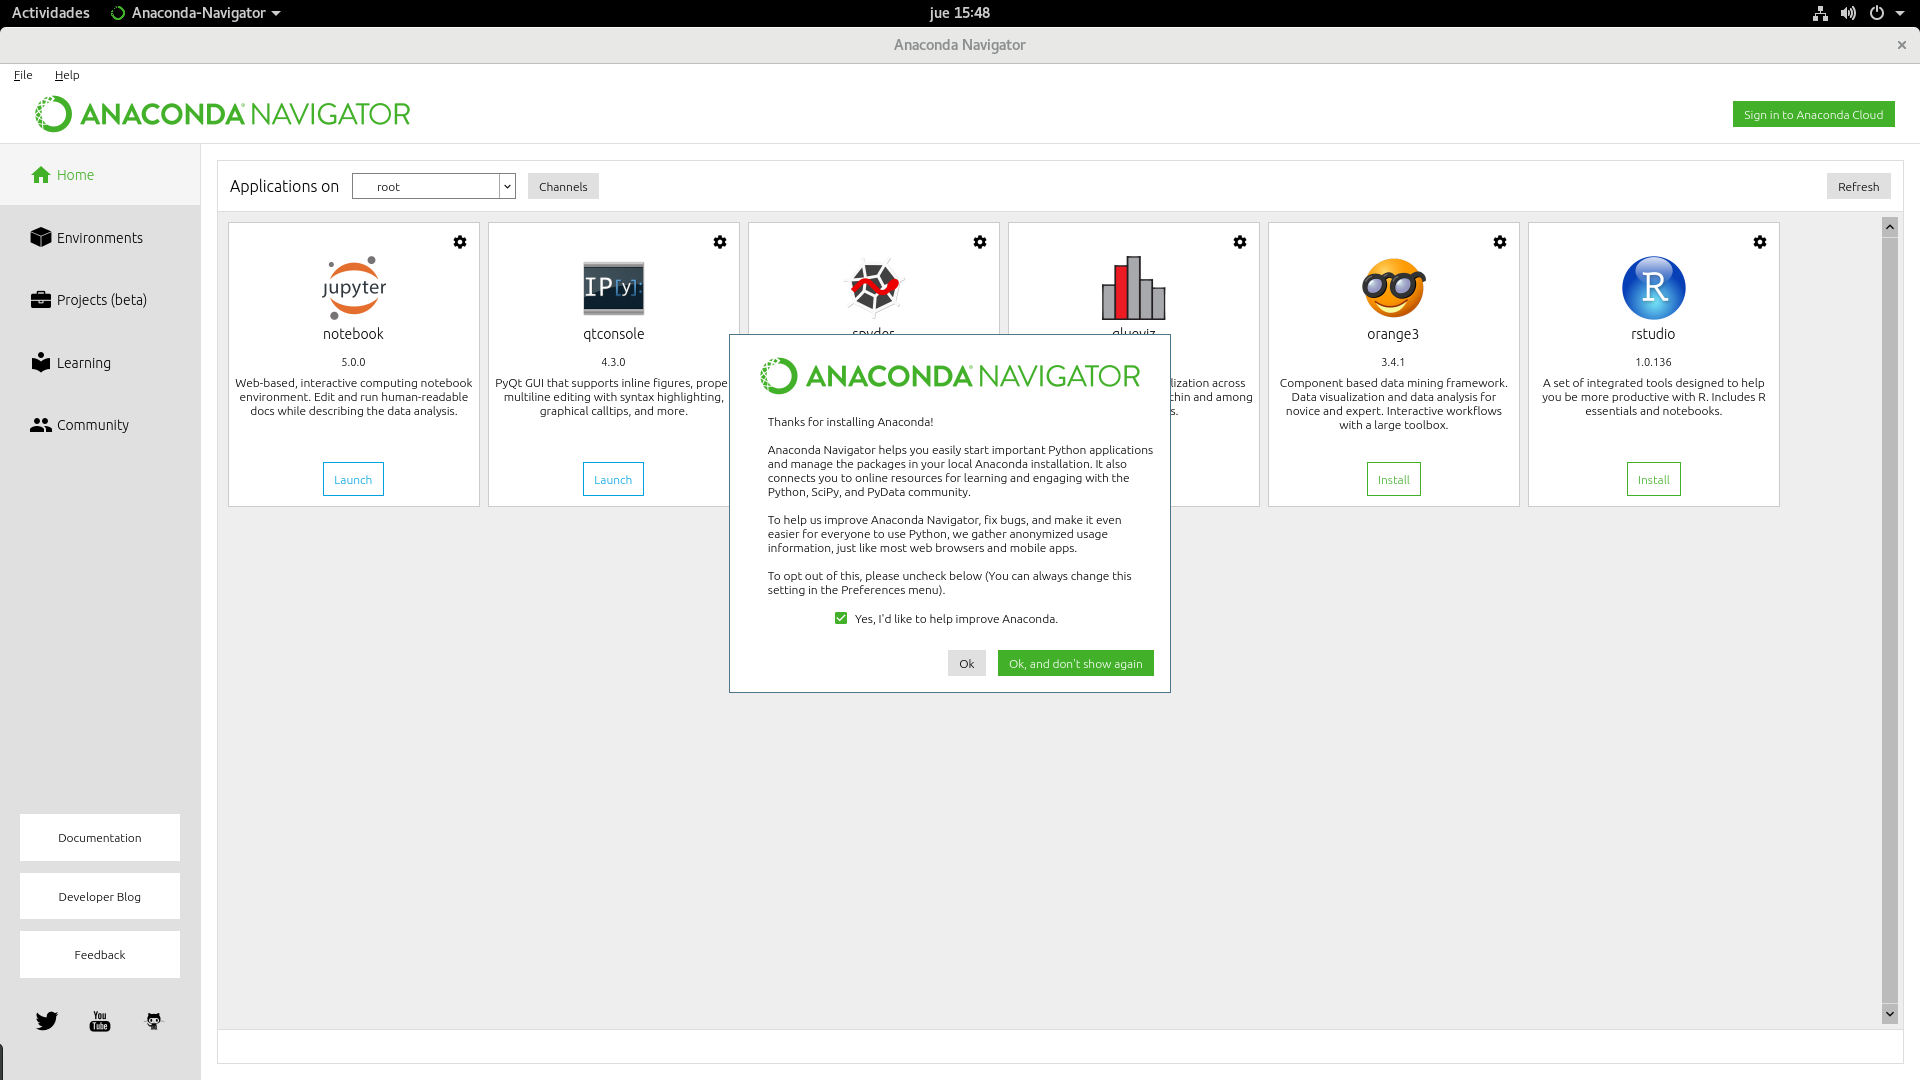
\includegraphics[scale=0.15]{Imagenes/Instalacion_Anaconda_01_linux_12}
\end{figure}
\end{enumerate}
\end{document}